\section{Reducción de Dimensión}\label{sec:reduccion}
Todo el análisis de esta sección se hizo con el conjunto de entrenamiento, y las evaluaciones usan los mismos 5 pliegues de la sección anterior, de modo que cada resultado se puede comparar con el modelo sin reducción mediante una prueba $t$ pareada.

\subsection{Análisis individual de variables}
Para medir la capacidad discriminativa de cada predictora por separado se usaron tres índices, con ``no reportado'' como una categoría más: la V de Cramér derivada de la prueba $\chi^2$ de independencia con la diabetes, que va de 0 a 1; la información mutua, y un AUC univariado, en el que cada categoría se reemplaza por la prevalencia de diabetes observada en ella (estimada fuera de pliegue). Con 274.031 registros las once pruebas $\chi^2$ resultan significativas ($p<0{,}01$), así que la decisión se basa en la magnitud de la asociación y no en el valor $p$.

\begin{figure*}[!t]
\centering
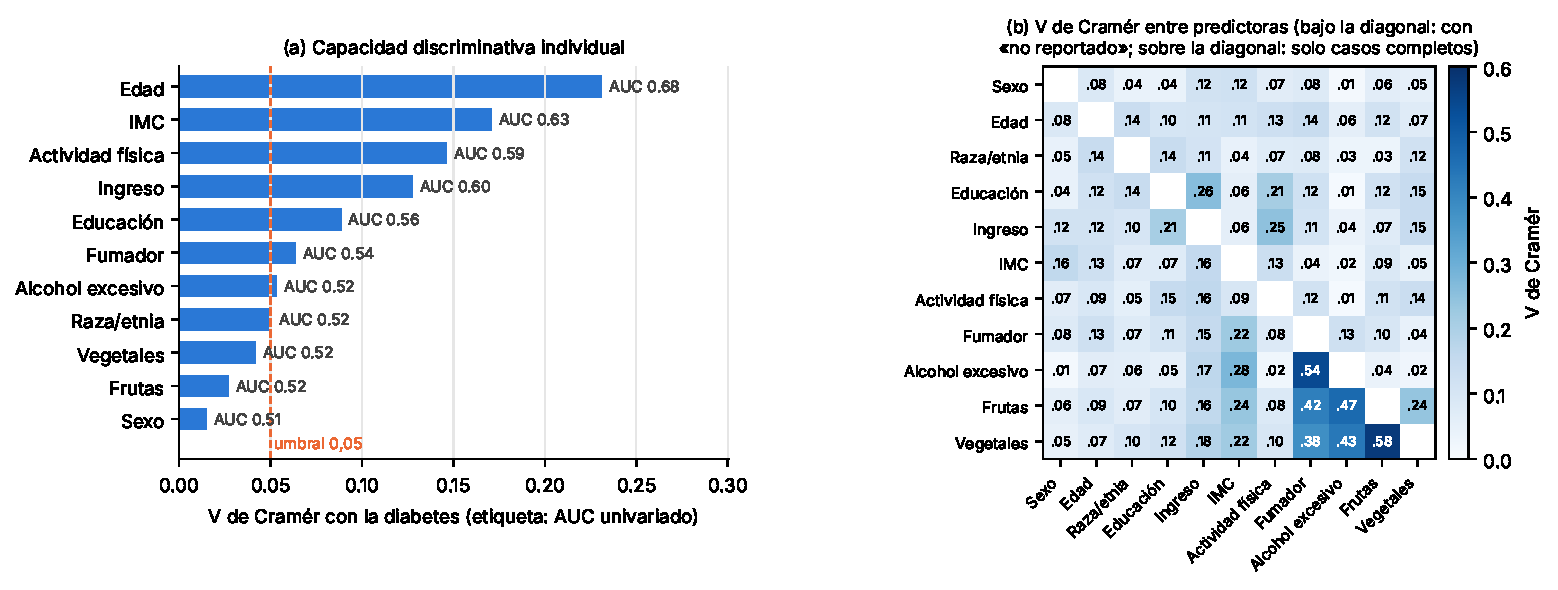
\includegraphics[width=0.9\textwidth]{analisis_individual.pdf}
\caption{(a) V de Cramér de cada predictora con la diabetes (barras) y su AUC univariado (etiqueta); la línea discontinua marca el umbral de 0,05 usado para señalar candidatas a eliminar. (b) V de Cramér entre pares de predictoras, calculada con ``no reportado'' como categoría (bajo la diagonal) y solo con los casos completos de cada par (sobre la diagonal).}
\label{fig:individual}
\end{figure*}

La Fig.~\ref{fig:individual}a ordena las variables. La edad es la más discriminativa por amplio margen (V = 0,23; AUC univariado de 0,68), seguida del IMC, la actividad física y el ingreso, lo que coincide con las variables de mayor peso que encontraron Majcherek et al. \cite{majcherek2025} con SHAP. En el otro extremo, vegetales, frutas y sexo tienen V por debajo de 0,05 y AUC univariados de 0,51 a 0,52, prácticamente el de una clasificación al azar. Con el criterio V $<0{,}05$ y AUC univariado $<0{,}55$, esas tres son las candidatas a eliminar; raza/etnia y alcohol quedan justo por encima del umbral.

La redundancia entre predictoras (Fig.~\ref{fig:individual}b) parece alta en algunos pares cuando se incluye ``no reportado'': frutas y vegetales tienen V = 0,58 y fumador y alcohol, 0,54. Sin embargo, con los casos completos esos valores bajan a 0,24 y 0,13. La asociación se debe sobre todo a que las mismas personas dejan sin responder varias preguntas de estilo de vida, no a que los hábitos se repitan entre sí. Ningún par supera 0,5 con casos completos, así que no se eliminó ninguna variable por redundancia.

Al retirar las tres candidatas, la regresión logística pasa de 57 a 49 columnas (14\% menos) y la SVM de 39 a 29 (26\% menos). El AUC de validación baja 0,12 pp en la regresión logística ($p=0{,}28$) y 0,20 pp en la SVM ($p=0{,}09$), diferencias que no son significativas, y la sensibilidad no cambia (Cuadro~\ref{tab:reduccion}). Vale la pena anotar que retirar solo el sexo de la SVM sí produce una caída pequeña pero significativa (0,25 pp; $p=0{,}04$): por sí solo casi no discrimina, pero el modelo no lineal parece aprovecharlo en combinación con otras variables, como el IMC.

\subsection{Extracción lineal de características: PCA}
PCA se insertó en el \textit{pipeline} justo después de la codificación, de modo que en cada pliegue los componentes se calculan solo con los datos de entrenamiento del pliegue. Para cada modelo se recorrió el número de componentes $k$ y se aplicó este criterio: el menor $k$ cuyo AUC de validación no sea significativamente menor que el del modelo sin reducción (prueba $t$ pareada, $p\geq0{,}05$) y cuya pérdida media no supere 0,5 pp. Se prefirió a un umbral fijo de varianza explicada porque en datos codificados la varianza no tiene por qué concentrarse en las direcciones que separan las clases, y aquí lo que importa es no perder capacidad de detección.

La Fig.~\ref{fig:pcaumap} muestra el resultado. En la regresión logística el AUC sube muy despacio con $k$: con 10 componentes, menos que las once variables originales, cae a 0,67, y el criterio solo se cumple con $k=45$ (AUC 0,76; $p=0{,}60$). Hay una razón estructural: las 57 columnas \textit{one-hot} suman 1 dentro de cada una de las once variables, así que su rango es 46, y 45 componentes equivalen casi al espacio completo. Además, la información de la edad, la variable más útil, está repartida en 14 columnas binarias de poca varianza cada una, y PCA, que solo atiende a la varianza, no tiene por qué conservarla en los primeros componentes. En la SVM, con edad, educación, ingreso e IMC como columnas estandarizadas, los primeros componentes sí recogen esa información: con 4 componentes el AUC ya es 0,74, y el criterio se cumple con $k=20$ (AUC 0,76; $p=0{,}35$; 98\% de la varianza), la mitad de las 39 columnas. Con $k=10$ la pérdida es de 1,09 pp y resulta significativa ($p<0{,}01$).

\begin{figure*}[!t]
\centering
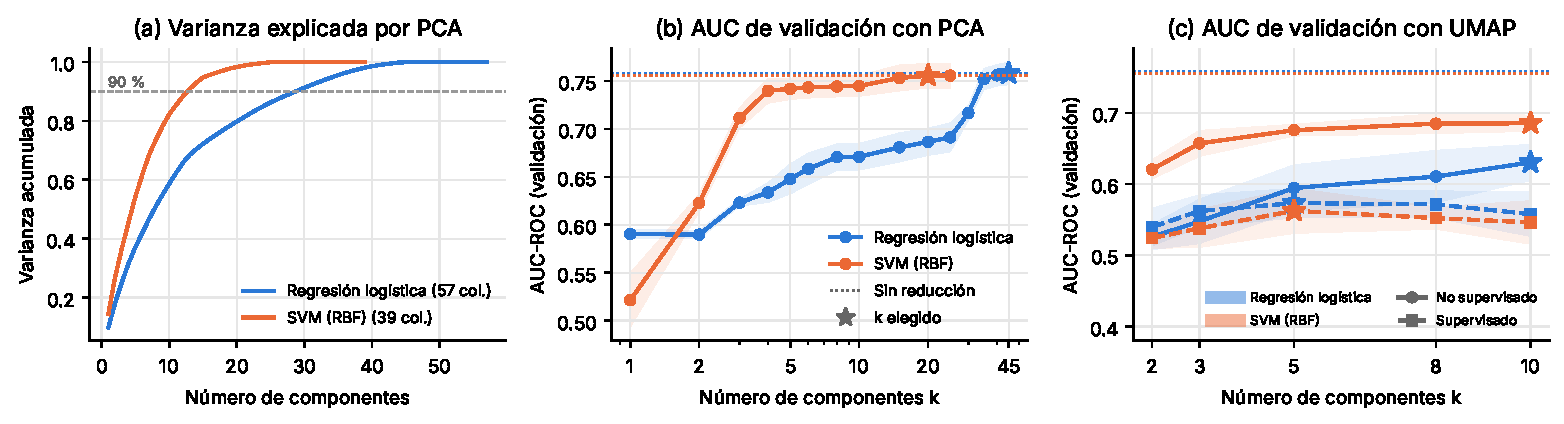
\includegraphics[width=0.92\textwidth]{pca_umap_componentes.pdf}
\caption{(a) Varianza explicada acumulada por PCA sobre la codificación de cada modelo. (b) y (c) AUC de validación (media e IC del 95\% en 5 pliegues) según el número de componentes con PCA y con UMAP; la línea punteada es el AUC sin reducción y la estrella marca el $k$ elegido con el criterio de no pérdida significativa.}
\label{fig:pcaumap}
\end{figure*}

\subsection{Extracción no lineal de características: UMAP}
UMAP construye un grafo de vecinos en el espacio codificado y busca una representación de baja dimensión que lo conserve. Se insertó en el mismo lugar del \textit{pipeline} que PCA, con \texttt{n\_neighbors} = 30, \texttt{min\_dist} = 0 (recomendado cuando el resultado se usa para clasificar y no para visualizar) y métrica euclidiana, y las coordenadas resultantes se estandarizaron antes del clasificador. Como la geometría cambia, se reajustó un hiperparámetro de cada modelo ($C\in\{0{,}01; 1\}$ en la regresión logística y $\gamma\in\{0{,}1;$ \texttt{scale}$\}$ en la SVM). Se recorrió $k\in\{2, 3, 5, 8, 10\}$, siempre por debajo de las once variables originales, con el mismo criterio de PCA. Además de la versión estándar, no supervisada, se probó UMAP supervisado, que al construir el grafo también usa la etiqueta, pero solo la de los registros de entrenamiento de cada pliegue; validación y prueba se proyectan sin etiqueta.

Ningún $k$ cumple el criterio (Fig.~\ref{fig:pcaumap}c). Con UMAP no supervisado el AUC de validación crece con $k$, pero con 10 componentes apenas llega a 0,63 en la regresión logística y 0,69 en la SVM, entre 7 y 13 pp por debajo del modelo sin reducción, así que se tomó $k=10$, el de mayor AUC. Una explicación probable es la naturaleza de los datos: once variables categóricas generan relativamente pocos perfiles distintos, con muchos registros idénticos, y el grafo de vecinos tiene que desempatar entre puntos a la misma distancia; además, UMAP conserva la estructura que domina el espacio codificado, que no tiene por qué ser la relacionada con la diabetes. La regresión logística sufre más porque el riesgo no es lineal en las coordenadas de UMAP, y el kernel RBF compensa una parte. La versión supervisada es peor todavía: el AUC de entrenamiento sube a 0,98, pero en validación no pasa de 0,57 y la sensibilidad cae por debajo de 0,20. El \textit{embedding} separa casi perfectamente a los registros de entrenamiento según su etiqueta, mientras que un registro nuevo, sin etiqueta, cae entre vecinos de ambas clases; es un sobreajuste del propio paso de reducción.

\begin{table*}[!t]
\centering
\caption{Desempeño de los dos mejores modelos con cada técnica de reducción. Dim.: número de columnas o componentes que recibe el clasificador; Red.: reducción frente a las columnas de la codificación original (57 en la regresión logística y 39 en la SVM). Entrenamiento y validación: media $\pm$ IC 95\% en 5 pliegues; prueba: valor con IC 95\% por \textit{bootstrap}}
\label{tab:reduccion}
\footnotesize
\setlength{\tabcolsep}{3.5pt}
\begin{tabular}{@{}lcccccccccc@{}}
\toprule
 & & & \multicolumn{3}{c}{\textbf{AUC-ROC}} & \multicolumn{2}{c}{\textbf{Sensibilidad}} & & \\
\cmidrule(lr){4-6} \cmidrule(lr){7-8}
\textbf{Versión} & \textbf{Dim.} & \textbf{Red.} & Ent. & Val. & Prueba & Val. & Prueba & \textbf{Espec.} & \textbf{F1} \\
\midrule
\multicolumn{10}{@{}l}{\textit{Regresión logística}} \\
\quad Sin reducción & 57 & -- & 0,76\,$\pm$\,0,00 & 0,76\,$\pm$\,0,01 & 0,77 [0,76; 0,77] & 0,75\,$\pm$\,0,01 & 0,75 [0,74; 0,76] & 0,65 & 0,40 \\
\quad Sin sexo, frutas y vegetales & 49 & 14\% & 0,76\,$\pm$\,0,00 & 0,76\,$\pm$\,0,01 & 0,77 [0,76; 0,77] & 0,75\,$\pm$\,0,02 & 0,74 [0,74; 0,75] & 0,65 & 0,40 \\
\quad PCA & 45 & 21\% & 0,76\,$\pm$\,0,00 & 0,76\,$\pm$\,0,01 & 0,77 [0,76; 0,77] & 0,75\,$\pm$\,0,01 & 0,75 [0,74; 0,76] & 0,65 & 0,40 \\
\quad PCA & 10 & 82\% & 0,67\,$\pm$\,0,00 & 0,67\,$\pm$\,0,01 & 0,68 [0,68; 0,69] & 0,60\,$\pm$\,0,02 & 0,62 [0,61; 0,63] & 0,65 & 0,34 \\
\quad UMAP & 10 & 82\% & 0,63\,$\pm$\,0,01 & 0,63\,$\pm$\,0,03 & 0,60 [0,60; 0,61] & 0,60\,$\pm$\,0,03 & 0,56 [0,55; 0,57] & 0,60 & 0,29 \\
\quad UMAP supervisado & 5 & 91\% & 0,98\,$\pm$\,0,00 & 0,57\,$\pm$\,0,02 & 0,62 [0,61; 0,62] & 0,10\,$\pm$\,0,02 & 0,18 [0,17; 0,18] & 0,92 & 0,22 \\
\multicolumn{10}{@{}l}{\textit{SVM (RBF)}} \\
\quad Sin reducción & 39 & -- & 0,77\,$\pm$\,0,00 & 0,76\,$\pm$\,0,01 & 0,77 [0,76; 0,77] & 0,78\,$\pm$\,0,01 & 0,80 [0,80; 0,81] & 0,60 & 0,40 \\
\quad Sin sexo, frutas y vegetales & 29 & 26\% & 0,76\,$\pm$\,0,00 & 0,75\,$\pm$\,0,01 & 0,76 [0,76; 0,77] & 0,78\,$\pm$\,0,01 & 0,80 [0,79; 0,81] & 0,60 & 0,39 \\
\quad PCA & 20 & 49\% & 0,76\,$\pm$\,0,00 & 0,76\,$\pm$\,0,01 & 0,77 [0,76; 0,77] & 0,78\,$\pm$\,0,01 & 0,80 [0,80; 0,81] & 0,60 & 0,40 \\
\quad PCA & 10 & 74\% & 0,75\,$\pm$\,0,00 & 0,74\,$\pm$\,0,01 & 0,76 [0,75; 0,76] & 0,77\,$\pm$\,0,01 & 0,81 [0,80; 0,82] & 0,57 & 0,38 \\
\quad UMAP & 10 & 74\% & 0,70\,$\pm$\,0,00 & 0,69\,$\pm$\,0,01 & 0,69 [0,69; 0,70] & 0,71\,$\pm$\,0,04 & 0,70 [0,69; 0,71] & 0,59 & 0,35 \\
\quad UMAP supervisado & 5 & 87\% & 0,98\,$\pm$\,0,00 & 0,56\,$\pm$\,0,03 & 0,55 [0,55; 0,56] & 0,08\,$\pm$\,0,01 & 0,14 [0,13; 0,14] & 0,95 & 0,19 \\
\bottomrule
\end{tabular}
\end{table*}

El Cuadro~\ref{tab:reduccion} reúne los resultados en prueba. Las tres versiones que no pierden desempeño en validación tampoco lo pierden en prueba: sin sexo, frutas y vegetales, con PCA de 45 componentes en la regresión logística y con PCA de 20 en la SVM, el AUC sigue en 0,76 a 0,77 y la sensibilidad en 0,74--0,75 y 0,80, respectivamente. Con 10 componentes, PCA le cuesta a la regresión logística 9 pp de AUC y 13 pp de sensibilidad, mientras que a la SVM solo 1 pp de AUC, con una sensibilidad similar (0,81) a cambio de 3 pp de especificidad. UMAP, en sus dos variantes, queda claramente por debajo, y la versión supervisada confirma en prueba el sobreajuste visto en validación (sensibilidad de 0,14 a 0,18).
